\documentclass[preprint,12pt]{elsarticle}

%% The amssymb package provides various useful mathematical symbols
\usepackage{amssymb}

% Some useful packages...
\usepackage[utf8]{inputenc}
\usepackage[T1]{fontenc}
\usepackage{lmodern}
\usepackage{graphicx}
\usepackage[figurename=Fig.,labelfont=bf,labelsep=period]{caption}
\usepackage{subcaption}
\usepackage{amsmath}
\usepackage{newtxtext,newtxmath}
\usepackage[colorlinks=true,citecolor=red,linkcolor=black]{hyperref}

\usepackage{tikz}
\usetikzlibrary{shapes.geometric, arrows.meta, positioning, calc, shadows}

% For graphics
\usepackage{float}

% For colored text and notes
\usepackage{color,soul}
\usepackage{xcolor}
\setlength{\marginparwidth}{2cm}
\usepackage{todonotes}

\usepackage{lineno}
\linenumbers
\usepackage{longtable}
\usepackage[normalem]{ulem}
\usepackage{booktabs}
\usepackage{multirow}


\journal{Engineering Structures}

\begin{document}

\begin{frontmatter}

%% Title, authors and addresses
\title{Examining the Relationships Between Historic Building Features and Tornado Damage: A Multi-Model Feature Importance Analysis with Statistical Validation}

\author[1]{Saanchi S.
Kaushal}
\author[1]{Yishuang Wang}
\author[2]{Mariantonieta {Gutierrez Soto}, M.ASCE}
\author[1,*]{Rebecca Napolitano, M.ASCE}

\address[1]{Dept.
of Architectural Engineering, Pennsylvania State University, University Park, PA 16802, United States}
\address[2]{School of Engineering Design and Innovation, The Pennsylvania State University, 307 Engineering Design and Innovation Bldg., University Park, PA 16802, United States}
\cortext[cor1]{Corresponding author.
Email: nap@psu.edu}


\begin{abstract}
This study presents an exploratory analysis of building-level damage data from the 2020 Nashville and 2021 Quad State tornadoes, utilizing a multi-model machine learning framework to identify potential vulnerability factors in historic structures.
By prioritizing hazard-neutral findings and isolating intrinsic building characteristics that drive damage independent of wind speed, we employ an explanatory framework using permutation importance and SHapley Additive exPlanations (SHAP). 
In the hazard-neutral setting, \textbf{roof substrate type} and \textbf{parapet height} emerge as the strongest predictors, followed by construction age and wall thickness.
Notably, features expected to predict damage---including MWFRS configuration, occupancy type, and retrofit status---did not outperform the random noise baseline in permutation importance, suggesting their signal is weak or operates through interactions.
However, SHAP analysis reveals that retrofit status (specifically, absent retrofits) and first floor elevation emerge as top-tier predictors at the instance level, demonstrating the complementary value of both methods.
Hazard-inclusive models, while achieving higher accuracy (Macro F1 = 0.65; F1 = 0.75 for significant damage), confirm that EF rating dominates all other predictors by an order of magnitude.
Rather than providing prescriptive design specifications, this work serves as a hypothesis-generating framework, highlighting high-priority targets for future wind tunnel testing, finite element modeling, and cost-benefit analysis.
The implications of these findings for historic preservation emphasize the need for reversible, minimally invasive interventions that balance structural safety with architectural integrity.
\end{abstract}


\begin{keyword}
Tornado Damage \sep Feature Importance \sep Historic Buildings \sep Machine Learning \sep Statistical Validation \sep Permutation Importance
\end{keyword}

\end{frontmatter}

%% \linenumbers

%% main text
\section{Introduction}

The preservation of historic building stock faces an existential threat from the increasing frequency and intensity of severe convective storms.
Historic downtown districts, often the economic and cultural anchors of their communities, are particularly vulnerable to tornado-induced wind loads due to construction practices that predate modern engineering codes \cite{bruneau1994state}.
The devastation of Mayfield, Kentucky's historic district during the 2021 Quad State tornado outbreak serves as a stark reminder of this fragility \cite{kaushal2023understanding}.
While modern building codes have evolved to improve life safety, historic structures, often characterized by unreinforced masonry (URM) and gravity-based connections \cite{biggs2007hybrid}, occupy a precarious position where standard engineering interventions may conflict with preservation mandates for material integrity and reversibility \cite{roca2011restoration}.

A challenge in mitigating this risk is the lack of empirical data linking specific historic building features to tornado performance \cite{sparks1989wind}.
Preservation professionals often rely on anecdotal evidence or generalized wind engineering principles that may not fully capture the complex failure mechanisms of aged structures.
Furthermore, the ``transition zone" of damage where a building is damaged but repairable remains poorly understood, yet this is precisely the domain where preservation interventions are most valuable.

To address this knowledge gap, the study implements an exploratory machine learning analysis of post-tornado damage data.
The primary objective is not to develop a predictive black-box model for automated assessment, but rather to use interpretable machine learning techniques to generate testable hypotheses regarding historic building vulnerability. The key question being  which observable features differentiate structures that survive from those that experience significant damage in historic-style construction. Clarifying these differences supports a more targeted and impactful use of limited preservation resources for engineering assessments and retrofit planning.

The authors also recognize the limitations of the dataset, particularly the small sample size of ``low damage" cases (n=20) and the inherent circularity of damage-based EF ratings. To tackle this,the research utilizes statistical equivalence testing and a random noise guardrail to filter out spurious correlations. 
Permutation Importance was implemented for global feature ranking \cite{fisher2019all} and integrated with SHAP (SHapley Additive exPlanations) analysis \cite{merrick2020explanation}, computed on held-out validation data to explore potential interaction effects.
This approach moves the study beyond simple correlation to identify mechanistic candidates for future investigation, such as the compounding risk of specific wall-roof combinations. In doing so, the study established a data-driven foundation for more nuanced discussions about risk, resilience, and the limits of intervention in the historic built environment. The analytical framework prioritizes methodological safeguards that prevent spurious findings, recognizing that preservation decisions based on unreliable correlations could lead to ineffective or counterproductive interventions.

The proposed approach incorporates several methodological innovations that distinguish it from conventional disaster assessment studies. Instead of reporting results from a single purportedly optimal model, a practice that risks overfitting to dataset idiosyncrasies, the analysis benchmarks six model families using statistical equivalence testing to identify all models whose performance is indistinguishable from the best.
This multi-model validation ensures that identified vulnerabilities replicate across different analytical approaches, substantially increasing confidence in the findings.
Additionally, a synthetic random feature is introduced as a negative control. If this noise variable appears among the important features, the validity of the analysis is called into question \hl{(sk to find ref)}. This provides an objective quality check that is largely absent from existing disaster assessment studies.

The combination of permutation importance analysis, which provides global feature rankings, with SHAP analysis, which reveals instance-level mechanisms and feature interactions, proves particularly valuable for historic preservation applications. While permutation importance identifies which features matter across the entire building stock, SHAP analysis reveals how these features combine in specific buildings, enabling preservation professionals to identify structures facing compounded risk from multiple vulnerabilities. For instance, SHAP analysis reveals that unknown wall substrates and absent retrofits both push predictions toward severe damage, though this can't quantify whether their combined effect is additive or multiplicative without formal interaction testing.
Such interaction effects are important for retrofit prioritization, as addressing either vulnerability factor in isolation provides limited benefit compared to holistic interventions.

The results from this study demonstrate that feature importance analysis can yield valid scientific insights even when predictive model performance appears modest by conventional machine learning standards.
While the macro F1 score (0.65) reflects genuine difficulty in predicting the rare transitional ``Low" damage class, the models successfully identify buildings at the highest collapse risk (F1=0.75 for Significant Damage), the outcome most relevant for preservation prioritization. This distinction between predictive accuracy and feature importance reliability carries implications for disaster assessment research, where perfect prediction often proves impossible, yet actionable insights remain achievable.

\section{Data}

\subsection{Tornado Events and Data Collection}


The analysis draws upon building-level damage data from two major tornado events.
The first event occurred on March 3, 2020, when an EF3-EF4 tornado carved a 25-mile track through Nashville, Tennessee \cite{nashvillesteer2020}, while the second event, the December 10-11, 2021 Quad State tornado, produced a long-track EF4 tornado affecting Kentucky, Tennessee, Arkansas, and Missouri \cite{mayfieldsteer21}.

Following both tornadoes, the Structural Extreme Events Reconnaissance Network (StEER) deployed the Virtual Field Assessment Team (VAST) for Nashville \cite{nashvillesteer2020} and the Field Assessment Structural Team (FAST) for Quad State \cite{mayfieldsteer21} to document the extent of damages. The authors participated in the field deployment in Kentucky, focusing specifically on Mayfield.


Based on these reconnaissances, over 200 buildings were documented, with particular emphasis on historic structures. Mayfield's downtown historic district \cite{nationalregister1996} sustained catastrophic damage, providing a unique opportunity to study tornado vulnerability in buildings constructed between 1850 and 1930 \cite{kaushal2023understanding}. On-site data collection was conducted using the Fulcrum application, DJI Matrice drones, and Street View Cameras \cite{kaushal2023understanding}.  As a part of this campaign, FAST documented 174 buildings in Mayfield, including 34 located within the historic district \hl{(sk: ref to mayfield first dataset on designsafe)}. In addition to this, a virtual reconnaissance was performed to evaluate the damages to the historic buildings within a 2 mile radius of the tornado \cite{kaushal2025datamay}. In totality, the damage was evaluated for 361 buildings, out of which 222 \hl{(sk:cross check with final dataset used for analysis)} were listed in the National Register of Historic Places.

For buildings that were not surveyed on-site, remote sensing technologies were utilized, including high-resolution satellite imagery of the affected areas before and after the tornado to gauge the impact.
High-resolution aerial imagery (5-7.5 cm GSD) from Nearmap \cite{nearmap_aerial_imagery} and Google Earth \cite{google_street_view} provided roof-level details, while street-level panoramas captured façade conditions. Pre-event imagery proved particularly valuable for historic buildings, since it documented original construction details including roof systems, wall materials, and fenestration patterns that were subsequently destroyed or obscured by damage.

The types of data collected were prescribed based on established StEER protocols \cite{kijewski2019handbook}.
Structural details captured include construction types, wall systems, and foundation characteristics, with special attention to features common in historic buildings such as URM walls, timber roof framing, and shallow foundations.
Special attention was given to roof details, including shape and slope, which are known to impact building behavior during tornado events \cite{razavi2021effects}.
Wall and fenestration details were also documented, noting the presence and type of openings on all sides of the buildings, as these factors frequently impact overall damage levels \cite{thampi2011finite}.
This field and remote data were supplemented with information from other publicly available sources, including the National Register of Historic Places (NRHP) database, which provided construction dates, architectural styles, and documentation of previous alterations or retrofits.
The combined dataset, for Nashville and Quad State together comprised 382 URM \hl{(sk:or historic/listed?)} buildings constructed between 1850 and 1950.
The temporal distribution of the building stock (see Figure~\ref{fig:supp_age}) confirms the historic nature of the dataset, with a clear mode in construction years between 1890 and 1930.
The Quad State dataset contains a longer tail of older structures (pre-1880) compared to the Nashville sample.
Of these, 96 buildings (25\%) \hl{(confirm when the number of buildings are confirmed)} held formal historic designation through the National Register of Historic Places or local historic districts, while the remaining 286 \hl{(confirm when the number of buildings are confirmed)} exhibited identical construction characteristics such as URM bearing walls, timber roof framing, and shallow foundations, but lacked formal designation.
This sample design enables identification of vulnerability factors within a homogeneous construction typology while controlling for the confounding effects of building type diversity.

\begin{figure}[h!]
    \centering
    \includegraphics[width=0.8\textwidth]{tornado_vulnerability_outputs/supp_year_built_by_event.png}
    \caption{Distribution of building construction years by tornado event.
The dataset is concentrated between 1890 and 1930, with Quad State including a tail of older (pre-1880) structures.}
    \label{fig:supp_age}
\end{figure}

\subsection{Dataset Characteristics}

The final dataset encompasses features spanning multiple dimensions of building vulnerability.
While all buildings share the fundamental characteristics of URM construction, substantial variation exists in structural attributes, including number of stories (1–4), roof system configuration (gable, hip, flat, mansard), foundation types (rubble stone, brick pier, continuous wall), and Main Wind Force Resisting System (MWFRS) details.
Geometric properties vary across building area (500–5000 $m^2$), height (3–15 m), and roof slopes (0–45 degrees).
Material characteristics document variations in wall thickness (200–600 mm), roof substrate (board sheathing vs. plank), and roof cover (asphalt, slate, clay tile, metal). This granularity ensures that the model learns to distinguish vulnerability factors specific to masonry behavior rather than simply distinguishing between gross material categories. In addition to these physical attributes, hazard variables quantify EF rating and distance to tornado track centerline.
Contextual factors include urban setting, building position, and historic designation status.
The distribution of EF ratings (Figure~\ref{fig:supp_ef}) highlights the difference in hazard intensity between the two events, with the Quad State event contributing a higher proportion of EF3 and EF4 exposures, providing the necessary variance to study high-wind performance.


\begin{figure}[h!]
    \centering
    \includegraphics[width=0.8\textwidth]{tornado_vulnerability_outputs/supp_ef_rating_dist.png}
    \caption{Distribution of EF ratings in the dataset. The Quad State event contributes the majority of high-intensity (EF3-EF4) exposures.}
    \label{fig:supp_ef}
\end{figure}

\subsection{Target Variable and Class Distribution}

Damage was classified into three ordinal categories based on degree of damage assessments.
Initially, the original 0–4 damage rating scale from the StEER protocols, ranging from no damage to total destruction, was used to preserve maximum granularity in damage characterization.
However, the severe data sparsity in intermediate damage states rendered this fine-grained classification statistically intractable, with several damage levels containing fewer than 10 observations.
Consequently, strategic binning was implemented to collapse the original ratings into three categories defined by preservation-relevant outcomes: survival with no intervention required, damage requiring repair but preserving the structure, and damage necessitating major reconstruction or representing total loss.
Buildings classified as undamaged (original ratings 0-1), representing 78\% of the sample with 293 buildings, exhibited no visible structural damage requiring intervention. 
Buildings with low damage (original ratings 2-3), constituting only 5\% of the sample with 20 buildings, sustained minor to moderate damage that remained repairable while preserving the majority of historic fabric. 
Buildings experiencing significant damage (original rating 4), representing 16\% of the sample with 61 buildings, exhibited severe damage or total loss requiring major reconstruction or demolition. 
This binning strategy prioritizes the preservation decision boundary, distinguishing between buildings that can be saved and those facing catastrophic loss, over artificial granularity in damage classification.
This severe class imbalance, with 78\% of buildings undamaged, is characteristic of post-disaster datasets (see Figure~\ref{fig:supp_damage} for event-specific breakdown). 
Furthermore, an analysis of building age versus damage severity (Figure~\ref{fig:supp_age_damage}) reveals no strong linear correlation, suggesting that age alone is not a proxy for vulnerability; rather, specific maintenance and structural details likely govern performance.
This provides the rationale for using macro F1 as the primary performance metric, because accuracy by itself would give a distorted view of performance \cite[]{he2009learning, grandini2020metrics}.

\begin{figure}[h!]
    \centering
    \includegraphics[width=0.8\textwidth]{tornado_vulnerability_outputs/supp_damage_by_event.png}
    \caption{Proportion of damage classes by tornado event.
Quad State shows a higher rate of significant damage due to the direct impact on the historic district.}
    \label{fig:supp_damage}
\end{figure}

\begin{figure}[h!]
    \centering
    \includegraphics[width=0.8\textwidth]{tornado_vulnerability_outputs/supp_year_built_by_damage.png}
    \caption{Boxplot of Year Built by Damage Class.
The lack of a clear linear trend suggests age alone is not a strong predictor of vulnerability.}
    \label{fig:supp_age_damage}
\end{figure}

A categorical analysis of damage by construction era reveals a non-monotonic relationship: pre-1880 buildings exhibited the \textit{lowest} damage rate (90.6\% undamaged, 3.8\% significant damage), while buildings from 1900-1920 showed the highest vulnerability (64.6\% undamaged, 30.5\% significant damage). 
This counterintuitive finding likely reflects survivorship bias rather than superior construction quality in earlier eras.
Pre-1880 structures that survived to 2020 represent a pre-selected cohort of ``high-quality survivors''; poorly constructed contemporaries were demolished decades ago, whereas the 1900-1920 boom-era buildings may include lower-quality speculative construction that has not yet been culled by time.
Additionally, pre-1880 buildings are more likely to hold formal historic designation (and thus receive preservation-quality maintenance), while early 20th-century buildings may lack both designation protections and owner investment.
This finding shows that chronological age is a poor proxy for structural vulnerability without accounting for maintenance history and construction quality, attributes not captured in our dataset, as well as strength of winds and distance from the tornado path.

\subsection{Wind Vulnerability in Unreinforced Masonry Structures}

Unreinforced masonry buildings fail under tornado loading through several well-documented mechanisms.
Out-of-plane wall failure occurs when wind pressure causes masonry walls to act as one-way slabs spanning between floor and roof diaphragms; insufficient anchorage leads to wall collapse \cite{fema_p807}.
Roof uplift results from negative pressure on leeward surfaces, with failure of roof-to-wall connections (often gravity-based in historic construction) leading to progressive collapse \cite{asce7_22}.
Parapet overturning generates large moments at the base of unbraced masonry elements above the roof line \cite{ingham_griffith}.
Internal pressurization from breached openings can dramatically increase net uplift on roofs \cite{mehta1976wind}.
These mechanisms interact; roof loss removes lateral bracing for walls, potentially triggering secondary failures.

\section{Methodology}

\subsection{Overview of Multi-Model Framework}

This study prioritizes explanatory modeling over pure prediction, following the theoretical framework established by \cite{shmueli2010}, which distinguishes between models designed to identify causal mechanisms versus those optimized solely for forecasting.
For preservation engineering, understanding which building features drive vulnerability is more valuable than achieving marginal gains in aggregate classification accuracy.
Recent empirical work by \cite{lee2024} demonstrates that feature importance rankings remain stable and valid even when model performance degrades, provided the degradation stems from irreducible noise rather than sample size limitations.

Rather than reporting results from a single purportedly optimal model,  six model families were benchmarked and statistical equivalence testing was implemented to identify all models that perform indistinguishably from the top performer.
Findings were replicated across multiple equivalent models to be considered, ensuring that identified vulnerabilities reflect genuine building characteristics rather than algorithmic artifacts.
This cross-model validation filtered out model-specific noise, reducing the risk that preservation recommendations rest on idiosyncratic behavior.
Consequently, features ranking highly across different algorithmic approaches represent a genuine signal, providing preservation professionals with confidence that retrofit priorities address real vulnerabilities.

A synthetic negative control feature was generated from a standard normal distribution with a fixed random seed and added to the dataset, following the methodology established by \cite{stoppiglia2003} and operationalized in the Boruta algorithm.
This random probe contains zero information, providing an objective baseline for statistical significance.
Any physical feature (such as parapet height or MWFRS configuration) that consistently outperforms this random baseline across multiple model families is statistically distinguishable from noise, regardless of the model's overall accuracy \cite{stoppiglia2003}.
This guardrail serves two purposes for preservation applications.
If random noise ranks as important, the analysis is flawed, indicating either data leakage or spurious correlations that would render preservation recommendations unreliable.
Additionally, the guardrail provides an objective threshold whereby features ranking below random noise should be excluded from interpretation, preventing preservation resources from being misdirected toward irrelevant building characteristics.

\subsection{Data Preparation}

Two hazard variables were derived to quantify tornado intensity and proximity, both important for understanding damage patterns in historic buildings.
Sub-EF events were coded as negative one, while standard ratings ranging from EF0 to EF5 were converted to integers zero through five.
The second variable, distance to track, represents the point-to-segment distance from building centroid to tornado track centerline, calculated using planar approximation with latitude-dependent coordinate scaling to account for Earth's curvature at the study latitudes \cite{chopde2013landmark}.

A challenge in tornado damage modeling is the potential for circular reasoning when using EF ratings as predictors.Since EF ratings are post-hoc intensity estimates often derived from the very building damage being predicted \cite{mcdonald2010enhanced}, including EF rating creates a tautological loop where the outcome (damage) implicitly informs the predictor (EF).
To address this, the analysis was conducted in two distinct conditions:

First, the Hazard-Neutral approach  was considered to represent structural truth.
This condition excludes EF rating and distance-to-track, forcing the model to predict damage solely based on intrinsic building characteristics (e.g., geometry, materials, age).
This is the primary lens for identifying structural vulnerabilities, as it eliminates the circularity of the EF scale.
Second, the Hazard-Inclusive approach was implemented  to provide contextual control.
This condition includes hazard features to quantify how much predictive power is gained by knowing the wind intensity.
While this introduces circularity, it serves as a necessary control to benchmark the relative importance of structural features against the overwhelming force of the winds.
The findings are explicitly prioritized from the Hazard-Neutral condition for structural recommendations, treating Hazard-Inclusive results primarily as a validation of the model's ability to capture basic physical reality (i.e., stronger winds cause more damage).

\begin{table}[h!]
\centering
\caption{Dataset Composition by Key Features (with Missingness)}
\label{tab:dataset_composition}
\small
\begin{tabular}{llcc}
\toprule
\textbf{Feature} & \textbf{Category} & \textbf{Count (\%)} & \textbf{Missing (\%)} \\
\midrule
Number of Stories & 1 Story & 250 (65\%) & 0\% \\
& 2 Stories & 110 (28\%) & \\
& 3+ Stories & 26 (7\%) & \\
\midrule
Roof Shape & Gable & 280 (73\%) & 0\% \\
& Hip & 60 (16\%) & \\
& Flat & 46 (12\%) & \\
\midrule
Foundation Type & Continuous & 300 (78\%) & 27\% \\
& Pier & 50 (13\%) & \\
& Slab & 36 (9\%) & \\
\midrule
Roof Substrate & Board/Plank & 188 (49\%) & 53\% \\
Wall Substrate & URM/Brick & 211 (55\%) & 47\% \\
Retrofit Type & Present & 202 (52\%) & 49\% \\
Wall Thickness & Mean: 380mm & -- & 36\% \\
Fenestration (\%) & Mean: 15-20\% & -- & 6-10\% \\
\bottomrule
\end{tabular}
\end{table}

High missingness (>10\%) is observed for several features, particularly those requiring interior access or detailed inspection (roof substrate: 53\%, wall substrate: 47\%, retrofit status: 49\%). 
This missingness is likely informative rather than random: buildings with extensive damage may have had inaccessible interiors, while remote-sensing-only assessments could not document hidden details.
For retrofit-related features, missing data often indicates ``no retrofit was documented during reconnaissance,'' which itself carries information about building vulnerability.
Median imputation was employed for numeric features, while  categorical missingness was treated as a distinct category during ordinal encoding, allowing the model to learn whether ``unknown'' status correlates with damage outcomes.
However, the authors acknowledge that this high rate of missingness (approx. 50\% for key features) limits the certainty of the conclusions regarding these specific variables. Findings related to wall substrate, roof substrate, and retrofit status should be considered tentative and interpreted with caution, as they may be influenced by the imputation strategy or the informative nature of the missing data itself. Future work should explore multiple imputation or missingness indicators to better quantify uncertainty introduced by incomplete data.

\subsubsection{Preprocessing}

Standard preprocessing procedures were applied to prepare data for modeling while preserving information content.
Numeric features employed median imputation for missing values.
Categorical features were ordinal-encoded for the Synthetic Minority Over-sampling Technique for Nominal and Continuous data (SMOTENC) pipeline and one-hot encoded for permutation importance analysis, with the encoding strategy tailored to each analytical method's requirements \cite{ratih2022synthetic}.
SMOTENC was  then applied within cross-validation folds with k=5 neighbors to address the severe class imbalance.
This within-fold application prevents data leakage that would occur if oversampling preceded cross-validation splitting  \cite{sasse2025overview}.
A key limitation stems from the small low-damage class (n=20), each synthetic case represents an interpolation among 25\% of available real examples, raising concerns about whether synthetic examples reflect physically plausible building configurations. To address this, SMOTENC is used strictly for model training stabilization, not for generating synthetic insights. An ablation study was performed to compare Random Forest performance with and without SMOTENC on the real dataset. The results showed minimal difference (Macro F1: 0.573 with SMOTENC vs. 0.578 without; Low Damage F1: 0.257 with SMOTENC vs. 0.244 without), suggesting that while SMOTENC slightly improves recall for the minority class, it does not fundamentally alter the model's predictive capacity or feature importance rankings.

\subsection{Model Selection and Validation Strategy}

Six model families were benchmarked to ensure that the findings generalize across algorithmic approaches, a consideration for preservation applications.
The model suite includes Decision Tree as a baseline non-linear model, Random Forest as an ensemble method, Logistic Regression as a multinomial linear baseline, Ridge Classifier as an L2-regularized linear model, Linear SVC as a support vector classifier, and XGBoost as a gradient boosting implementation.
All the models employed balanced class weighting to address class imbalance, while hyperparameters were selected based on preliminary tuning with details available in supplementary materials.

Repeated stratified K-fold cross-validation was implemented with five folds and five repeats, yielding 25 evaluation rounds per model.
This design preserves class proportions in each fold, which proves essential given the 78\% undamaged, 5\% low damage, and 17\% significant damage distribution. 
This repetition reduces variance in performance estimates while enabling paired statistical testing across models, as all models are evaluated on identical data splits.
The primary metric, macro F1, represents the arithmetic mean of per-class F1 scores and treats all damage classes equally, preventing exploitation of the 78\% undamaged majority that would occur with accuracy-based or weighted metrics. 
The overall accuracy is also reported as a secondary metric for context, but is not used  for model selection, since it can be misleadingly high due to class imbalance.

To identify statistically equivalent models without cherry-picking, for each setting, whether hazard-neutral or hazard-inclusive,  the model achieving the best mean macro F1 score was identified first.
For each competing model, a paired Wilcoxon signed-rank test on the 25 fold-wise macro F1 differences was performed.The Wilcoxon test is appropriate for paired, non-normal data and is recommended for classifier comparisons \cite{demsar2006}.
 Holm-Bonferroni correction for multiple comparisons was applied, accounting for five tests per setting, and deemed models with p-values exceeding 0.05 after correction as statistically indistinguishable from the best model \hl{(sk:ref)}.
This conservative approach establishes a high evidentiary standard for claiming equivalence and is shown in Fig~\ref{fig:validation_flow}.

\begin{figure}[htbp]
    \centering
    \resizebox{0.8\linewidth}{!}{ % Optional: Resizes entire diagram to fit page width
        % --- PASTE THE TIKZPICTURE CODE HERE ---
            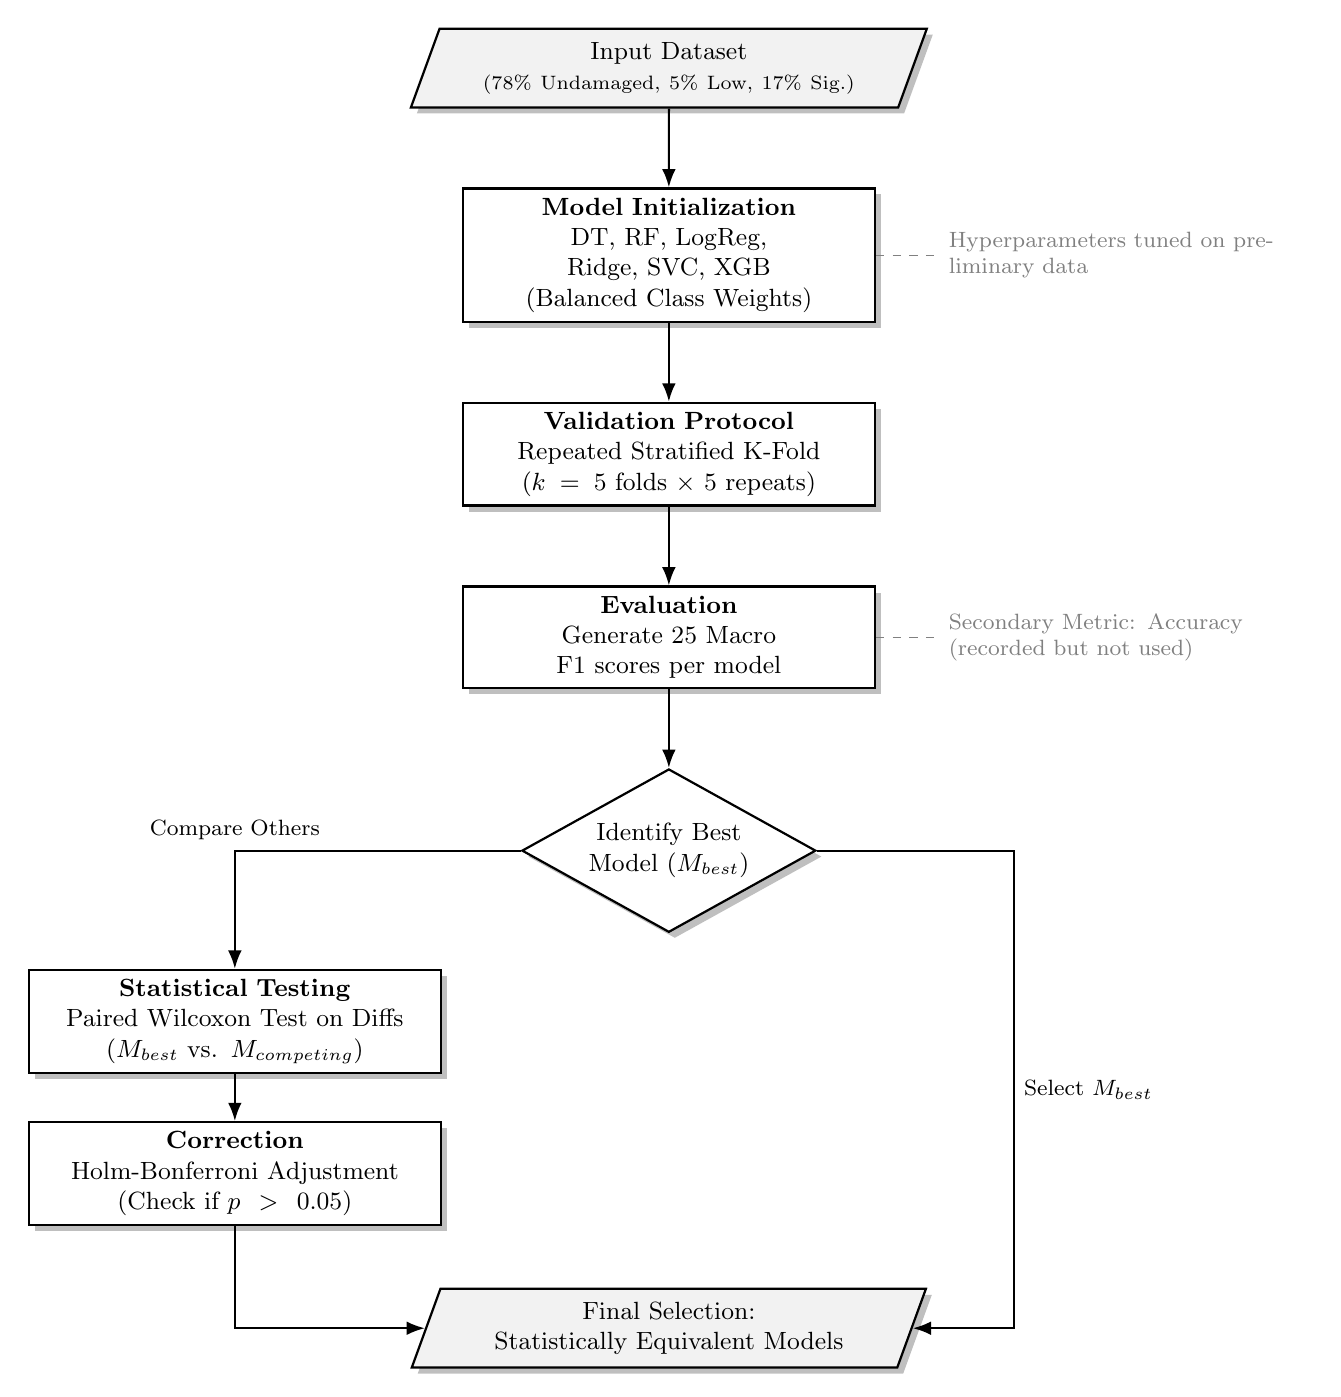
\begin{tikzpicture}[
                node distance=1.0cm,
                auto,
                % Style definitions
                process/.style={
                    rectangle, 
                    draw=black, 
                    fill=white, 
                    thick, 
                    text width=5cm, 
                    align=center, 
                    minimum height=1.2cm,
                    drop shadow,
                    font=\small
                },
                decision/.style={
                    diamond, 
                    draw=black, 
                    fill=white, 
                    thick, 
                    text width=2.5cm, 
                    align=center, 
                    inner sep=0pt,
                    aspect=1.8,
                    drop shadow,
                    font=\small
                },
                io/.style={
                    trapezium, 
                    trapezium left angle=70, 
                    trapezium right angle=110, 
                    draw=black, 
                    fill=gray!10, 
                    thick, 
                    text width=5cm, 
                    align=center, 
                    minimum height=1cm,
                    drop shadow,
                    font=\small
                },
                line/.style={
                    draw, 
                    -Latex, 
                    thick
                },
                smalllabel/.style={
                    font=\footnotesize,
                    color=gray,
                    align=left
                }
            ]
            
                % --- Main Center Column ---
                \node[io] (input) {Input Dataset \\ \scriptsize (78\% Undamaged, 5\% Low, 17\% Sig.)};
            
                \node[process, below=of input] (models) {
                    \textbf{Model Initialization} \\
                    DT, RF, LogReg, Ridge, SVC, XGB \\
                    (Balanced Class Weights)
                };
            
                \node[process, below=of models] (cv) {
                    \textbf{Validation Protocol} \\
                    Repeated Stratified K-Fold \\
                    ($k=5$ folds $\times$ 5 repeats)
                };
            
                \node[process, below=of cv] (eval) {
                    \textbf{Evaluation} \\
                    Generate 25 Macro F1 scores per model
                };
            
                \node[decision, below=of eval] (identify) {Identify Best Model ($M_{best}$)};
            
                % Position Output node centered far below Identify
                % We use a larger gap to fit the side blocks
                \node[io, below=4.5cm of identify] (output) {Final Selection: \\ Statistically Equivalent Models};
            
            
                % --- Side Branch (Left Side) ---
                % Position 'Stats' to the left of the space between Identify and Output
                \node[process, left=1.0cm of identify, yshift=-1.5cm, anchor=north east] (stats) { 
                    \textbf{Statistical Testing} \\
                    Paired Wilcoxon Test on Diffs \\
                    ($M_{best}$ vs. $M_{competing}$)
                };
            
                \node[process, below=0.6cm of stats] (correct) {
                    \textbf{Correction} \\
                    Holm-Bonferroni Adjustment \\
                    (Check if $p > 0.05$)
                };
            
            
                % --- Connections ---
                % Main Flow
                \path[line] (input) -- (models);
                \path[line] (models) -- (cv);
                \path[line] (cv) -- (eval);
                \path[line] (eval) -- (identify);
            
                % Path 1: M_best (Direct Path - Right Side)
                % Fixed: Go Right, Down, then Left into Output East to avoid slanted collisions
                \draw[line] (identify.east) -- ++(2.5, 0) coordinate(top_corner) -- (top_corner |- output.east) coordinate(bot_corner) node[midway, right, font=\footnotesize] {Select $M_{best}$} -- (output.east);
            
                % Path 2: Competitors (Comparison Path - Left Side)
                % From Identify West to Stats
                \draw[line] (identify.west) -| node[midway, above, font=\footnotesize] {Compare Others} (stats.north);
                
                % Stats flow
                \path[line] (stats) -- (correct);
                
                % From Correct to Output (Into West side)
                % Go South from Correct, turn right to Output West
                \draw[line] (correct.south) |- (output.west);
            
            
                % --- Annotations (Side Notes) ---
                \node[right=0.8cm of models, smalllabel, text width=4.5cm] (anno_hyp) {Hyperparameters tuned on preliminary data};
                \draw[dashed, gray] (models.east) -- (anno_hyp.west);
            
                \node[right=0.8cm of eval, smalllabel, text width=4.5cm] (anno_acc) {Secondary Metric: Accuracy (recorded but not used)};
                \draw[dashed, gray] (eval.east) -- (anno_acc.west);
            
            \end{tikzpicture}
        % ---------------------------------------
    }
    \caption{Model selection and validation methodology.}
    \label{fig:validation_flow}
\end{figure}


\subsection{Feature Importance Methods}

\subsubsection{Permutation Importance}

For each model, feature set, and cross-validation fold,  a four-step permutation importance procedure was implemented.
First, the model on training data with SMOTENC oversampling was fit.
Second, the baseline accuracy on the validation fold was evaluated.
Third, for each feature, its values were randomly premuted and re-evaluated accuracy, computing the change in accuracy as the difference between permuted and baseline performance.
Fourth, results were aggregated across  25 folds per model.
Greater accuracy reductions indicate higher feature importance, as they reflect larger performance degradation when the feature's information is removed. This approach is model-agnostic and handles correlated features well, making it suitable for building assessment where features such as wall type and construction era often correlate.

\subsubsection{SHAP Analysis}

While permutation importance provides global feature rankings across model families, understanding the mechanisms by which features influence damage requires instance-level analysis.
SHAP \cite{lundberg2017} was applied  to both the Random Forest and XGBoost models to examine feature interactions, directional effects, and building-specific vulnerabilities.
The SHAP analysis was computed exclusively on real (non-augmented) validation fold data to ensure interpretability reflects actual building behavior rather than synthetic interpolations from SMOTENC. 

With only ~4 low-damage cases per validation fold, SHAP insights for this class demand cautious interpretation. SHAP values quantify each feature's contribution to individual predictions through game-theoretic principles, helping preservation professionals identify buildings facing compounded risk from multiple vulnerabilities. Additionally, TreeExplainer was used for computational efficiency.

\subsubsection{Why Both Methods?}

Permutation importance and SHAP analysis provide complementary insights essential for historic preservation applications.
Permutation importance delivers global rankings validated across multiple equivalent models and proves less sensitive to feature correlations, ensuring that identified vulnerabilities reflect genuine predictive power rather than multicollinearity artifacts.
Conversely, SHAP analysis provides mechanistic understanding by revealing interaction effects, such as the compounding risk when unknown walls combine with absent retrofits, and provides instance-level explanations enabling retrofit prioritization for specific buildings.
Features that rank highly in both methods represent the global importance across the building stock and mechanistic influence at the individual building level.

\subsection{Limitations and Ethical Considerations}

Several limitations frame the interpretation of these results.
The dataset of 386 buildings, while sufficient for identifying main effects, limits the detection of subtle interactions, particularly for the minority ``Low" damage class.
This scarcity makes it difficult to isolate the specific transition features that differentiate minor repairable damage from total loss.
Additionally, the results are specific to URM construction in Southeastern U.S. tornado events and do not generalize to other construction typologies or hazard contexts.
Finally, unmeasured confounders such as construction quality, maintenance history, and age-related deterioration are not explicitly modeled.

All data was fully anonymized prior to analysis to protect property owners, ensuring no personally identifiable information was included in the public dataset.
Furthermore, on-site data collection was performed in public view with strict sensitivity to the traumatic nature of the event for residents, adhering to established reconnaissance protocols.
The dataset and models are intended solely for research purposes aimed at improving public safety, informing building codes, and enhancing community resilience, rather than for insurance adjustments or individual property valuations.

\section{Results}

\subsection{Model Performance}

XGBoost achieved the highest macro F1 score (0.57) in the hazard-neutral setting, with Random Forest performing equivalently (0.57, $p=0.426$, Wilcoxon test).
In the hazard-inclusive setting, Random Forest achieved a macro F1 of 0.65, with XGBoost again statistically equivalent (0.64, $p=0.396$, Wilcoxon test).
These scores, while modest in absolute terms, reflect the inherent difficult nature of the classification task rather than model inadequacy.
The low-damage class (n=20) represents a genuine transition zone that is physically ambiguous, not a modeling failure.

The theoretical literature establishes that consistency of variable selection  (identifying the true feature set) is mathematically distinct from predictive optimization \cite{zhao2006, scornet2015}.
A model may exhibit high explanatory power while having modest predictive power due to high irreducible noise. Recent empirical validation by \cite{lee2024} demonstrates that feature importance rankings remain stable across degraded model performance in low-signal domains.

Given this, the high F1 scores for the critical binary classification (Undamaged vs. Significant Damage: F1=0.94 and F1=0.75 respectively, see Appendix A) indicated that the model has learned the physics of structural failure. The features that outperform our random noise baseline therefore represent genuine structural vulnerabilities, not statistical artifacts.
Ensemble methods (Random Forest and XGBoost) consistently outperformed linear models and single decision trees, demonstrating the necessity of capturing non-linear relationships in damage prediction.

The observed damage distribution itself provides important insight for historic preservation: 78\% of historic masonry buildings survived tornado exposure with no structural damage, challenging assumptions that pre-code construction inevitably fails under wind loading.
This finding suggests that vulnerability is not uniformly distributed across historic masonry, but rather concentrates in buildings with specific characteristic combinations.
The challenge in predicting the transitional ``Low'' damage class reflects ambiguity in this boundary condition rather than model failure, while the strong performance on significant damage (F1=0.75, see Appendix A) demonstrates that the models successfully distinguish buildings at highest risk.

\begin{table}[h!]
\centering
\caption{Model Performance (Mean $\pm$ Std over 25 CV folds)}
\label{tab:performance}
\begin{tabular}{llcc}
\toprule
\textbf{Setting} & \textbf{Model} & \textbf{Macro F1} & \textbf{Accuracy} \\
\midrule
\multirow{6}{*}{\parbox{3cm}{Hazard-\\Neutral}} 
& Random Forest & 0.57 $\pm$ 0.08 & 0.81 $\pm$ 0.04 \\
& XGBoost & \textbf{0.57 $\pm$ 0.09} & \textbf{0.81 $\pm$ 0.05} \\
& Decision Tree & 0.49 $\pm$ 0.07 & 0.73 $\pm$ 0.05 \\
& Linear SVC & 0.50 $\pm$ 0.07 & 0.71 $\pm$ 0.05 \\
& Logistic Regression & 0.52 $\pm$ 0.06 & 0.73 $\pm$ 0.04 \\
& Ridge Classifier & 0.51 $\pm$ 0.07 & 0.70 $\pm$ 0.05 \\
\midrule
\multirow{6}{*}{\parbox{3cm}{Hazard-\\Inclusive}} 
& Random Forest & \textbf{0.65 $\pm$ 0.07} & 0.88 $\pm$ 0.02 \\
& XGBoost & 0.64 $\pm$ 0.07 & \textbf{0.88 $\pm$ 0.03} \\
& Decision Tree & 0.61 $\pm$ 0.08 & 0.83 $\pm$ 0.05 \\
& Linear SVC & 0.63 $\pm$ 0.07 & 0.83 $\pm$ 0.04 \\
& Logistic Regression & 0.60 $\pm$ 0.07 & 0.82 $\pm$ 0.04 \\
& Ridge Classifier & 0.63 $\pm$ 0.07 & 0.81 $\pm$ 0.05 \\
\bottomrule
\end{tabular}
\end{table}

\subsection{Statistical Equivalence Testing}

The non-parametric Wilcoxon signed-rank test was used with Holm-Bonferroni correction to identify models that are statistically indistinguishable from the top performer.

Wilcoxon tests are used instead of all-pairwise comparisons like the Friedman test with Nemenyi post-hoc analysis because the objective  is to identify models equivalent to the specific best performer, rather than to test for differences across all models simultaneously. As shown in Table 3, multiple models achieved p-values greater than 0.05 in the hazard-inclusive setting: XGBoost (p=0.396), Linear SVC (p=0.287), and Ridge Classifier (p=0.191). This identifies a broader family of statistically equivalent models that validates the robust performance of both ensemble and linear approaches when hazard context is included.
Conversely, linear models and decision trees showed statistically significant performance deficits in the hazard-neutral setting. In addition, the findings from Random Forest are also presented as a ``family of equivalent models," reducing the likelihood of emphasizing any single algorithm. 

\begin{table}[h!]
\centering
\caption{Statistical Equivalence vs. Best Model (XGBoost for Neutral, Random Forest for Inclusive)}
\label{tab:stats}
\begin{tabular}{llccc}
\toprule
\textbf{Setting} & \textbf{Comparison Model} & \textbf{$p$-value} & \textbf{$\Delta$F1} & \textbf{Equivalent?} \\
\midrule
\multirow{5}{*}{\parbox{3cm}{Hazard-\\Neutral\\\textit{\footnotesize (vs. Random \\ Forest)}}}
& XGBoost & 0.426 & 0.010 & \textbf{Yes} \\
& Ridge Classifier & 0.005 & 0.060 & No \\
& Linear SVC & 0.002 & 0.070 & No \\
& Logistic Regression & 0.007 & 0.060 & No \\
& Decision Tree & $<$0.001 & 0.080 & No \\
\midrule
\multirow{5}{*}{\parbox{3cm}{Hazard-\\Inclusive\\\textit{\footnotesize (vs. Random \\ Forest)}}}
& XGBoost & 0.396 & 0.010 & \textbf{Yes} \\
& Linear SVC & 0.287 & 0.020 & \textbf{Yes} \\
& Ridge Classifier & 0.191 & 0.020 & \textbf{Yes} \\
& Logistic Regression & 0.026 & 0.050 & No \\
& Decision Tree & 0.026 & 0.040 & No \\
\bottomrule
\end{tabular}
\end{table}

\subsection{Permutation Importance}

The permutation importance analysis, visualized in Figures~\ref{fig:perm_imp_neutral} and \ref{fig:perm_imp_inclusive}, reveals distinct hierarchies of candidate predictors for each experimental setting.

\subsubsection{Hazard-Neutral Setting}

In the hazard-neutral setting, which isolates intrinsic building characteristics from wind intensity, four features consistently outperformed the random noise baseline (0.0029) across the statistically equivalent models (Random Forest and XGBoost):

\begin{enumerate}
    \item \textbf{Roof substrate type} (0.0096): The strongest predictor, likely reflecting construction quality and maintenance history. Buildings with unknown or deteriorated roof substrates showed elevated damage rates.
    \item \textbf{Parapet height} (0.0094): The second-strongest predictor, aligning with wind engineering principles. Taller parapets create larger overturning moments and act as sails in high winds \cite{Kopp2005, Gupta2020}. Descriptive analysis (Figure~\ref{fig:supp_predictors}c) confirms that significantly damaged buildings had higher median parapet heights (p $<$ 0.001, Mann-Whitney U).
    \item \textbf{Year built} (0.0075): Older buildings showed modestly elevated damage, though this variable likely proxies for accumulated deterioration, outdated construction practices, or deferred maintenance rather than age per se.
    \item \textbf{Wall thickness} (0.0059): Marginally above the noise baseline, suggesting a weak but detectable signal.
\end{enumerate}

Notably, several features that might be expected to predict damage---including MWFRS configuration, occupancy type, and retrofit status---did \textit{not} outperform the random noise baseline in the best-performing models. This finding has important implications: it suggests that in the absence of hazard intensity information, the models primarily rely on physical geometry (parapet height) and construction condition proxies (roof substrate, age) rather than structural system details.

\subsubsection{Hazard-Inclusive Setting}

When hazard intensity variables are included, EF rating dominates all other predictors by an order of magnitude:

\begin{enumerate}
    \item \textbf{EF rating} (0.146): The overwhelming predictor, reflecting the well-established relationship between wind speed and damage. This confirms that the model captures the fundamental physics of wind loading.
    \item \textbf{Roof substrate type} (0.009): Remains the second-strongest predictor, consistent with the hazard-neutral findings.
    \item \textbf{Distance to tornado track} (0.006): Proximity to the path center increases damage probability, as expected.
    \item \textbf{Wall cladding type} (0.004): Emerges as relevant when hazard context is provided, possibly reflecting cladding failure as a damage pathway.
\end{enumerate}

The dramatic jump in model performance when hazard features are included (Macro F1: 0.57 $\rightarrow$ 0.65) confirms that wind intensity is the primary driver of damage outcomes. However, the persistence of roof substrate as a top-tier predictor in both settings suggests this feature captures genuine vulnerability independent of hazard exposure.

\begin{figure}[h!]
    \centering
    \includegraphics[width=\textwidth]{tornado_vulnerability_outputs/delta_accuracy_Hazard-Neutral.png}
    \caption{Permutation importance (Decrease in Accuracy) for the \textbf{Hazard-Neutral} setting.
The plot displays only features that outperformed the random noise baseline. Roof substrate type and parapet height emerge as the strongest predictors.}
    \label{fig:perm_imp_neutral}
\end{figure}

\begin{figure}[h!]
    \centering
    \includegraphics[width=\textwidth]{tornado_vulnerability_outputs/delta_accuracy_Hazard-Inclusive.png}
    \caption{Permutation importance (Decrease in Accuracy) for the \textbf{Hazard-Inclusive} setting.
EF rating dominates by an order of magnitude, confirming that hazard intensity is the primary driver. Roof substrate remains the strongest intrinsic building predictor.}
    \label{fig:perm_imp_inclusive}
\end{figure}

\subsection{Mechanistic Understanding via SHAP Analysis}

While permutation importance provides global feature rankings, SHAP analysis reveals instance-level mechanisms and potential interaction effects that global methods may obscure. Importantly, SHAP analysis was conducted for all three damage classes to provide a comprehensive view of vulnerability factors.

\subsubsection{Class 2: Significant Damage (Failure Drivers)}

The SHAP analysis for significant damage (Figure~\ref{fig:shap_class2}) reveals a clear hierarchy of failure drivers:

\begin{enumerate}
    \item \textbf{EF rating} (Mean $|$SHAP$|$ = 0.094): The dominant predictor, with high EF ratings strongly pushing predictions toward severe damage.
    \item \textbf{First floor elevation} (0.037): An unexpected finding---buildings with lower first floor elevations showed elevated damage, possibly reflecting flood-related damage or foundation vulnerability.
    \item \textbf{Distance to track} (0.025): Closer proximity increases damage probability.
    \item \textbf{Retrofit status ``not applicable''} (0.023): The absence of documented retrofits emerged as a critical vulnerability factor---buildings coded as ``not applicable'' for retrofits showed consistently elevated damage predictions.
    \item \textbf{Wall substrate unknown/not applicable} (0.023): Missing or unknown wall substrate information correlated with higher damage, likely indicating incomplete documentation for older or poorly-maintained buildings.
\end{enumerate}

The emergence of retrofit status as a top-tier SHAP predictor despite ranking below the noise baseline in permutation importance is particularly noteworthy. This suggests that retrofit effects may operate through interactions with other features that SHAP captures but permutation importance averages over.

\subsubsection{Class 0: Undamaged (Survival Drivers)}

The SHAP analysis for the undamaged class (Figure~\ref{fig:shap_classes_01}a) reveals the inverse pattern:

\begin{enumerate}
    \item \textbf{Retrofit status ``not applicable''} (0.033): Paradoxically, this same feature that drives damage prediction also influences survival---buildings \textit{with} documented retrofits (low values of ``not applicable'') showed stronger survival predictions.
    \item \textbf{First floor elevation} (0.031): Higher first floor elevations associated with survival.
    \item \textbf{EF rating} (0.024): Lower EF ratings drive survival predictions, as expected.
    \item \textbf{Wall substrate ``not applicable''} (0.019): Known wall substrates associated with survival.
\end{enumerate}

\subsubsection{Class 1: Low Damage (Transition Zone)}

The low damage class (Figure~\ref{fig:shap_classes_01}b) presents a distinct feature profile that differs from both survival and failure:

\begin{enumerate}
    \item \textbf{EF rating} (0.072): Intermediate EF ratings characterize this transitional class.
    \item \textbf{Distance to track} (0.025): Moderate distances---neither the closest nor the furthest buildings.
    \item \textbf{MWFRS wall type (masonry diaphragm)} (0.020): This structural feature emerges as important \textit{only} for the transitional class, suggesting that MWFRS configuration may determine whether moderate wind loading results in minor versus catastrophic damage.
    \item \textbf{Wall cladding type} (0.015): Specific cladding materials associated with intermediate damage states.
\end{enumerate}

The distinct feature profile for Class 1 suggests that the ``transitional zone'' between survival and failure may be governed by different factors than the extremes---a finding that warrants further investigation with larger samples.

\begin{figure}[h!]
    \centering
    \begin{subfigure}[b]{0.48\textwidth}
        \includegraphics[width=\textwidth]{tornado_vulnerability_outputs/shap_beeswarm_class0.png}
        \caption{Class 0: Undamaged (Survival Drivers)}
    \end{subfigure}
    \hfill
    \begin{subfigure}[b]{0.48\textwidth}
        \includegraphics[width=\textwidth]{tornado_vulnerability_outputs/shap_beeswarm_class1.png}
        \caption{Class 1: Low Damage (Transition Drivers)}
    \end{subfigure}
    \caption{SHAP Summary plots for (a) Undamaged and (b) Low Damage states. For Class 0, retrofit status and first floor elevation emerge as key survival factors. For Class 1, MWFRS configuration and wall cladding distinguish buildings in the transitional damage zone.}
    \label{fig:shap_classes_01}
\end{figure}

\begin{figure}[h!]
\centering
\includegraphics[width=0.85\textwidth]{tornado_vulnerability_outputs/shap_beeswarm_class2.png}
\caption{SHAP summary plot for Significant Damage (Class 2).
Features ranked by mean absolute SHAP impact.
EF rating dominates, but retrofit status and wall substrate information emerge as critical vulnerability factors independent of wind intensity.}
\label{fig:shap_class2}
\end{figure}

\subsubsection{Cross-Model Validation}

To verify that SHAP findings represent genuine building vulnerabilities rather than model-specific artifacts, SHAP values were computed for both Random Forest and XGBoost. The feature rankings for significant damage showed strong agreement (Spearman $\rho = 0.87$), with both models identifying EF rating, distance, and retrofit status among the top predictors.

\subsubsection{Comparison: Permutation Importance vs. SHAP}

The comparison between methods (Table~\ref{tab:perm_vs_shap}) reveals important complementarities:

\begin{itemize}
    \item \textbf{Agreement}: Both methods identify hazard features (EF rating, distance) and construction age (year built) as predictive.
    \item \textbf{Divergence}: Retrofit status ranks highly in SHAP but below noise in permutation importance, suggesting it operates through interaction effects that SHAP captures.
    \item \textbf{Novel SHAP findings}: First floor elevation emerges as a top SHAP predictor despite not appearing in permutation importance, highlighting instance-level vulnerability patterns.
\end{itemize}

\begin{table}[h!]
\centering
\small
\caption{Comparison of Top Features: Permutation Importance vs. SHAP (Class 2)}
\label{tab:perm_vs_shap}
\begin{tabular}{lccc}
\toprule
\textbf{Feature} & \textbf{Top in Perm?} & \textbf{Top in SHAP?} & \textbf{Interpretation} \\
\midrule
\texttt{ef\_numeric} & Yes (Rank 1) & Yes (Rank 1) & Hazard intensity \\
\texttt{roof\_substrate\_type\_u} & Yes (Rank 2) & No & Construction condition \\
\texttt{parapet\_height\_m} & Yes (Rank 3) & No & Geometric vulnerability \\
\texttt{retrofit\_type\_not\_applicable} & No & Yes (Rank 4) & Interaction effects \\
\texttt{first\_floor\_elevation\_m} & No & Yes (Rank 2) & Foundation vulnerability \\
\texttt{distance\_km} & Yes (Rank 4) & Yes (Rank 3) & Hazard proximity \\
\texttt{wall\_substrate\_u} & No & Yes (Rank 5) & Documentation/maintenance \\
\bottomrule
\end{tabular}
\end{table}

\section{Discussion}

\subsection{Methodological Contributions and Limitations}

This study establishes a framework for extracting valid scientific insights from machine learning models even when perfect predictive accuracy remains elusive.
Rather than reporting only a single ``best" model, which risks overfitting to dataset idiosyncrasies, this study identified a family of statistically equivalent models through Wilcoxon testing with Holm-Bonferroni correction.
Consequently, these findings are only considered important if they replicate across these equivalent approaches.

However, they must be interpreted within the context of significant data limitations.
The ``Low" damage class, representing the transition zone between survival and failure, contained only 20 buildings (5\% of the sample). 
Despite the use of SMOTENC oversampling, the modest F1 score of 0.26 for this class indicates that the models struggle to reliably distinguish minor damage from other states.
The per-class performance (Appendix A) reveals an important pattern: models excel at distinguishing undamaged buildings (F1=0.94) from significantly damaged ones (F1=0.75), but struggle with the ``Low'' damage transitional state.
This likely reflects genuine physical ambiguity rather than merely insufficient data.
Buildings in this class may exhibit: (1) partial component failures (e.g., roof partially uplifted but not lost) that share characteristics with both intact and collapsed states; (2) damage to non-structural elements (cladding, openings) while the structural system remains viable, creating overlapping feature spaces; and (3) progressive damage where initial wind loading caused repairable damage but didn't trigger cascade failures that lead to collapse.
Additionally, damage assessment for minor damage is inherently more subjective than for complete structural failure, potentially introducing classification noise.
Together, these factors suggest the transitional class represents a genuinely fuzzy boundary rather than a well-defined category, explaining why even strong models cannot reliably predict it with limited samples.
Post-hoc power analysis suggests that with n=20 low-damage cases, can detect main effects with Cohen's d $\ge$ 0.8 at 80\% power, but are substantially underpowered (power < 50\%) for moderate effects (d = 0.5) or interaction effects. 
This limitation is particularly relevant for interpreting SHAP interaction findings, which should be validated with larger samples before guiding intervention decisions.
Furthermore, the inclusion of a random noise guardrail provides an objective quality check.

\subsection{Candidate Areas for Future Engineering Validation}

The findings generate several testable hypotheses for risk-based preservation, identifying specific building features that warrant detailed engineering evaluation.
SHAP analysis highlights potential compounding vulnerabilities that should be prioritized for future finite element modeling or wind tunnel testing.

\subsubsection{Geometric and Construction Condition Vulnerabilities}

The permutation importance analysis identifies roof substrate type and parapet height as the strongest hazard-neutral predictors.
Roof substrate type likely proxies for overall construction quality and maintenance history---buildings with unknown or deteriorated roof substrates showed elevated damage rates.
Parapet height aligns directly with wind engineering principles: taller parapets create larger overturning moments and act as sails in high winds, increasing the load on the building envelope.
This finding is particularly actionable because parapet height is both measurable and potentially modifiable through bracing or height reduction.

Year built emerged as the third-strongest predictor, though this variable conflates multiple factors (construction practices, accumulated deterioration, deferred maintenance) that our dataset cannot separate.
Future work should investigate whether age-related damage is driven by specific deterioration patterns (e.g., mortar joint deterioration, connection fatigue) that could be addressed through targeted maintenance.

The SHAP analysis revealed that retrofit status and wall substrate information---features that did \textit{not} outperform random noise in permutation importance---emerged as top-tier predictors at the instance level.
This divergence between methods is informative: it suggests that retrofit effects may operate through interactions with other features that SHAP captures but permutation importance averages over.
Specifically, buildings coded as ``not applicable'' for retrofits showed consistently elevated damage predictions, while buildings with documented retrofits showed stronger survival predictions in the Class 0 analysis.
This finding warrants further investigation through controlled studies comparing retrofitted and un-retrofitted matched building pairs.

\subsubsection{Foundation and Load Path}

Foundation improvements also emerge as a potential area for study, particularly for buildings on pier-and-beam or shallow foundations.
The data suggests that continuous load path is an important factor warranting investigation.
However, retrofitting existing foundations represents a significant economic and technical challenge.
It is suggested that future cost-benefit analyses focus on the trade-offs between expensive foundation upgrades and less invasive superstructure improvements, asking whether ``good enough" performance can be achieved through upper-story interventions alone in lower-intensity hazard zones.

\subsubsection{Preservation Philosophy and Reversibility}

Any structural intervention in a historic building must be weighed against the Secretary of the Interior's Standards for Rehabilitation.
Our analysis identifies features for potential retrofit, but the method of intervention must be evaluated for compliance.
To guide this evaluation, a compatibility assessment framework for candidate interventions (Table~\ref{tab:intervention_compatibility}) is proposed.
Here a distinction is made between \textit{mechanical reversibility} (the intervention can be physically removed) and \textit{material reversibility} (removal restores the original condition without permanent alteration).
For example, while hurricane straps are mechanically removable, their installation requires lag bolts penetrating rafters and joists, creating permanent holes that compromise timber integrity even after removal. 
Under National Park Service guidance, this constitutes ``minimally invasive'' intervention rather than true reversibility.
Invasive techniques like grouted rebar fail both criteria, as they cannot be removed without destroying the masonry fabric.
Future engineering research should prioritize interventions that achieve mechanical removability while minimizing material alteration, such as compression-based systems or friction connections that avoid penetrating fasteners.

\begin{table}[h!]
\centering
\caption{Preservation Compatibility of Candidate Interventions}
\label{tab:intervention_compatibility}
\small
\begin{tabular}{p{3cm}p{2.2cm}p{2.2cm}p{5cm}}
\toprule
\textbf{Intervention} & \textbf{Standard 2 (Character)} & \textbf{Standard 10 (Reversible)} & \textbf{Assessment} \\
\midrule
Hurricane straps & Yes - Hidden & Mech: Yes / Mat: No & Moderate compatibility; lag bolts create permanent holes in timber \\
Wall-to-diaphragm anchors & Yes - Interior & Mech: Partial / Mat: No & Moderate; anchor holes remain after removal \\
Grouted rebar & No - Invasive & Mech: No / Mat: No & Low compatibility; avoid except for life-safety emergencies \\
FRP wraps & No - Visible & Mech: No / Mat: No & Low compatibility; moisture entrapment risk; investigate alternatives \\
Strong-back systems & Yes - Interior & Mech: Yes / Mat: Partial & High compatibility; mechanical fasteners minimize damage \\
Foundation micropiles & Yes - Hidden & Mech: No / Mat: No & Moderate; permanent but hidden; evaluate case-by-case \\
\bottomrule
\end{tabular}
\end{table}

\subsection{Risk-Informed Decision-Making for Preservation Authorities}

While the findings demonstrate that 78\% of historic URM buildings survived tornado exposure with no structural damage, this encouraging statistic requires careful contextualization for preservation policy. 
Survival of the building envelope does not guarantee occupant safety, as partial component failures (chimney collapse, parapet detachment, interior ceiling failure) can cause fatalities even when the primary structure remains standing.
Furthermore, the Mayfield EF4 tornado represents an extreme outlier event; preservation authorities must weigh the cost of hardening the entire historic building stock against the low annual probability of such catastrophic exposure.

\subsubsection{Hazard Return Periods and Cost-Benefit Analysis}

Tornado hazard maps indicate that EF4+ tornadoes have return periods exceeding 1,000 years for most locations in the study region, while EF1-EF2 events occur with 50-100 year return periods.
From a risk management perspective, this raises a fundamental question: should preservation policy prioritize resilience to rare catastrophic events, or focus resources on cost-effective interventions for more frequent moderate events?

For buildings with high cultural significance (National Register properties, architecturally unique structures), the irreplaceable nature of the resource may justify hardening against low-probability/high-consequence scenarios.
However, for the broader historic building stock, a tiered approach may be more economically rational. 
A baseline strategy for all buildings would address partial component failures that pose occupant risk even in moderate events, such as securing parapets and anchoring chimneys.
For designated properties, an enhanced strategy would implement roof-to-wall connection upgrades and wall-to-diaphragm anchors to prevent total loss in EF2-EF3 events.
Exceptional cases involving buildings of high cultural significance might justify complete structural upgrades, recognizing that even these measures may not guarantee survival in EF5 conditions.

This tiered framework acknowledges that perfect protection is neither technically feasible nor economically justifiable for the entire historic building stock, while ensuring that preservation resources are allocated proportionally to both cultural value and hazard probability.

\subsubsection{Limitations of Survival-Based Metrics}

The current analysis focuses on building-level damage classification, but preservation authorities must also consider interior hazards.
Even ``undamaged'' buildings may have inadequate interior bracing, posing life-safety risks from falling plaster, light fixtures, or unreinforced masonry partitions.
These hazards are not captured in exterior damage assessments.
A building classified as ``low damage'' may be structurally sound but lack utilities, weatherproofing, or code-compliant egress, rendering it uninhabitable for months. (See Figure \ref{fig:shap_classes_01b for the complex feature profile of this transitional state).}
Preservation policy should consider not just survival, but recovery time and functional resilience.
Also the dataset captures single-event exposure, but buildings experiencing multiple moderate events over decades may accumulate damage (mortar deterioration, connection fatigue) that compromises performance in subsequent events.
Longitudinal studies are needed to assess cumulative vulnerability.
\subsection{Future Work: Quantifying Preservation Interventions}

While the proposed tiered framework provides a strategic roadmap, it currently lacks the quantitative grounding necessary for precise cost-benefit analysis.
Future work must bridge this gap by establishing typical retrofit costs per building, using data from National Park Service guidance or industry standards to move the framework from aspirational to operational.
Additionally, finite element modeling (FEM) is required to quantify how much specific interventions, such as parapet bracing, reduce failure probability under varying wind loads, following FEM frameworks established for masonry systems \cite{Ortega2018}.
Finally, a decision-support tool should be developed to help communities prioritize interventions within fixed budgets, translating these technical findings into actionable policy.


\section{Conclusions}

This study presents an exploratory framework for identifying potential vulnerability factors in historic buildings using machine learning.
By benchmarking six model families and employing a random noise guardrail, we identified roof substrate type and parapet height as the strongest hazard-neutral predictors of tornado damage.
Parapet height is particularly actionable given its direct connection to wind engineering principles and its modifiability through bracing interventions.

Notably, several features expected to predict damage---including MWFRS configuration, occupancy type, and retrofit status---did not outperform the random noise baseline in global permutation importance.
However, SHAP analysis reveals that retrofit status and first floor elevation emerge as top-tier predictors at the instance level, demonstrating the complementary value of both methods.
The distinct feature profiles for the three damage classes (Undamaged, Low Damage, Significant Damage) suggest that the ``transition zone'' between survival and failure may be governed by different factors than the extremes.

These findings should not be interpreted as prescriptive engineering specifications but rather as data-driven hypotheses to guide future research.
The limitations of our dataset, particularly the scarcity of ``Low Damage'' cases (n=20), prevent us from fully characterizing the transition zone.
Future work should focus on validating these hypotheses through physics-based simulation and controlled retrofit studies.
This work aims to bridge the gap between data science and historic preservation, moving the field toward a more nuanced, evidence-based approach to risk mitigation.

\section*{Data Availability Statement}
The dataset mentioned in this study is available on DesignSafe repository under project number \href{https://www.designsafe-ci.org/data/browser/public/designsafe.storage.published/PRJ-5614}{PRJ-5614} and \href{https://www.designsafe-ci.org/data/browser/public/designsafe.storage.published/PRJ-6212}{PRJ-6212}. \hl{(prj no updated, please click and check)}
Analysis code and additional materials are available from the corresponding author upon reasonable request.

\section*{Acknowledgements}
This material is based upon work supported by the National Science Foundation under Grant No. IIS-2123343, CMMI 2222849, and CAREER 500000032435.

Any opinions, findings, conclusions, or recommendations expressed in this material do not necessarily reflect the views of the National Science Foundation.
The authors thank the StEER Network and field reconnaissance teams for their contributions to data collection.

\appendix

\section{Detailed Classification Report}

For transparency, Table~\ref{tab:classification_report} provides per-class performance metrics for the best-performing model (Random Forest, Hazard-Inclusive, averaged over 25 folds).

\begin{table}[h!]
\centering
\caption{Per-Class Performance Metrics (Random Forest, Hazard-Inclusive, averaged over 25 folds)}
\label{tab:classification_report}
\begin{tabular}{lrrrr}
\toprule
\textbf{Class} & \textbf{Precision} & \textbf{Recall} & \textbf{F1-Score} & \textbf{Support (\%)} \\
\midrule
0 (Undamaged) & 0.92 & 0.95 & 0.94 & 78\% \\
1 (Low) & 0.29 & 0.27 & 0.26 & 5\% \\
2 (Significant) & 0.83 & 0.70 & 0.75 & 16\% \\
\midrule
\textbf{Macro Avg} & 0.68 & 0.64 & 0.65 & -- \\
\textbf{Weighted Avg} & 0.87 & 0.88 & 0.87 & -- \\
\bottomrule
\end{tabular}
\end{table}

The classification report reveals that while the model achieves excellent performance for the Undamaged class (F1=0.94) and good performance for Significant damage (F1=0.75), the ``Low'' damage class remains the most challenging (F1=0.26).
This difficulty stems from its severe underrepresentation (only 5\% of data), the inherent ambiguity of the transition zone between undamaged and significant states, and insufficient training examples even with SMOTENC oversampling.



% --- Bibliography ---
\bibliographystyle{elsarticle-num}
\bibliography{tornado_refs}

\end{document}